\chapter{概率与统计 - 贝叶斯统计\&机器学习分类指标}
\begin{figure}[ht]
  \centering
  \includegraphics[width=1\linewidth]{asset/茶桁的 AI 秘籍_Math_22.png}
\end{figure}
\newpage


今天让我们来学习一下「贝叶斯统计」和「机器学习分类指标」, 这两部分结束之后, 咱们《概率和统计》的部分就结束了. 不知道这段时间的内容对大家是否有帮助. 

好, 咱们正课走起. 

\section{贝叶斯统计}

贝叶斯是非常厉害的一个人, 在统计学里面贝叶斯做出了太多的贡献. 就包括在概率里面, 有频率派, 也有贝叶斯派. 当然在机器学习里面, 也有贝叶斯派. 就是从贝叶斯的角度去考虑机器学习的模型, 和神经网络的连接主义是对立的关系. 

说到贝叶斯统计, 肯定绕不开贝叶斯公式, 一个大数学家、统计学家提出的这么一个公式. 以他命名的公式如下: 

\[P(Y|X) = \frac{P(X|Y)P(Y)}{P(X)}\]

这个式子特别简单,就是由条件概率和联合概率的公式得到的. 为什么能得到这个式子?咱们把分母$P(X)$乘到式子左边去, 左边$P(Y|X) \cdot P(X)$, 不就是 X 和 Y 的联合概率嘛. 等式左右两边都是一个联合概率, 所以把$P(X)$拿到右边作为分母, 这个式子就出来了. 就是这么简单, 贝叶斯公式就是这么简单. 

我们来看一下这个公式里面各个量的一些含义. 按照贝叶斯的语言, X 代表了可被观测到的样本. 观测到的这个样本就是可以看见了, 可以统计出来, 可以数出来的. 比如抛硬币, 正面朝上多少次, 反面朝上多少次, 这个可观测到的. 

然后, Y 代表了产生这个样本的内在机制的参数, 或者说产生这个样本的概率模型的这么一个参数, 就比如说均值方差. 如果这个模型不是你自己设计出来的, 只是去观察它的话是无法单纯的通过观察观察出来的, 你是看不出来的, 但是它是客观存在的. Y 就是这种概率模型的参数. 大家可以理解为均值, 方差那一类的东西. 很多教科书往往说到这些参数的时候, 并没有指明这个参数是什么东西. 很多人在学的时候就会非常云里雾里的, 都不知道参数是啥, 我咋往下去看呢. 

接着$P(Y|X)$称为后验概率 $(\mathord{posterior})$, 我们先来看一下这个$P(Y)$, $P(Y)$称为先验概率$(\mathord{prior})$. 一个是先验一个是后验, 它们俩的区别是一个有$|X$一个没有$|X$, 这个也体现了贝叶斯派的一个思维模式. 这个这部分内容我们待会也会讲到. 就是频率派是只关注观测到的样本, 但是贝耶斯派说不行, 我们在处理这些样本之前需要对这个样本背后的概率模型有一个先验性的一个预判, 或者说预估. 

打比方说, 一个人去称体重, 他大概知道自己几斤几两, 大概知道自己的身体体重范围. 可能是在 120 斤~140 斤之间. 这个就是先验的分布的一种预估. 他知道自己是落在这个范围内了, 这个就是一种预估. 

所以贝耶斯派说必须要先弄一个先验的分布, 这样子才能安心的去做事情. 如果你就是闷头闷耳去研究这个样本而对先验的一个预估都没有的话, 这个做着不放心. 贝耶斯派干事是这个样子的. 

那为什么$P(Y|X)$被称为这个后验概率了. 后验概率和先验概率有什么不一样?后验概率多了一个$|X$. 我们知道这是一个条件概率对不对, 这个条件概率告诉了我们在 X 已知或者说被观测到的前提下, 我对 Y 所做的一个预估. 所以它叫做后验. 

因为先验是我们还没有处理样本 X 的时候, 人为去设想的. 这个设想可以有理论性的依据, 也可以是人主观的臆断. 

大家注意, 在这里先验分布是可以有主观臆断的. 就比如如果你实在没辙了, 从理论分析不出来这个到底是怎么一回事. OK, 那你自己按照你主观的判断, 按照主观的意愿去设一个都行, 但是你不能没有. 

$P(Y|X)$为什么叫后验概率呢?就是因为我们已经掌握了样本, 在掌握了样本之后
我们再对这个参数的分布去做一个调整. 这个时候叫做后验概率. 

$P(X)$叫做证据$(\mathord{evidence})$,这个用处往往不是特别的大. 这个可能就代表了我用记忆学习模型去做一些分类, 或者说去做这个情感分析, 在所有的这些数据里面, 积极的、乐观的这个情感是有多少条. 消极的、愤怒的情感是有多少条. 这个被称为证据. 往往相对于其它三个用处不是特别的大. 

然后还有一个$P(X|Y)$, 叫做自然估计, 自然估计也是非常重要的一个概念. 不要看着它很简单, 就是一个条件概率模型, 但是我们在机器学习里面, 尤其是很多传统机器学习模型, 比如高斯混合模型, 就用到的这种最大自然估计. 

最大自然估计中, 首先这个 X 是我们已经确定的样本. Y 是我们现在所设想, 或者说待优化的概率模型的参数, 比如说均值或者说方差. 

接下来我们来打比方, 打比方说我们考虑高斯分布的这种情形有一些数据点. 比如说我给了 3 个数据点, 我们看一下图\ref{fig:img23_1}: 

\begin{figure}[ht]
  \centering
  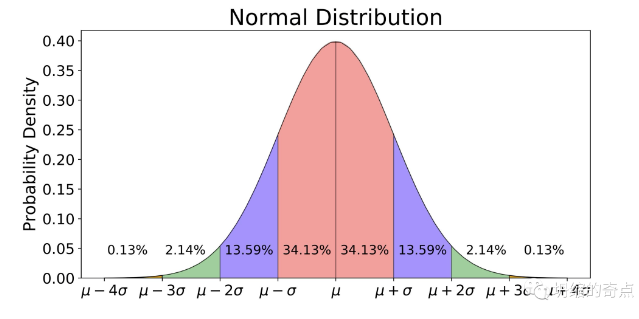
\includegraphics[width=1\linewidth]{asset/20231227144618.png}
  \caption{}
  \label{fig:img23_1}
\end{figure}

在这个图上面, 个顶点的那个位置各挑了 3 个点, 总共这三个点给到你, 这个就是我们的样本 X. 然后我们可以得到什么样的结论?
首先我们已经知道了, 这个模型是一个高斯模型, 或者说我们觉得高斯模型去做这个拟合效果会比较好. 

那现在问题就来了, 即便是选中的三个点, 我们同样是用高斯分布去做, 那他们也有很多不同的高斯分布可以满足经过这三点. 就像二次函数里面随机挑两个点, 另外一个二次函数也有可能经过这两个点一样, 它是一个多值的情况. 

在这种情况下我们怎么样判断哪一个高斯分布是最优的一个解呢?这个时候就用到了刚才说的, 最大自然估计. 

我们再来看一下最大自然估计, 在 Y 的前提 X 发生的概率, 所以用在我们刚才所说的这个例子里面. 比如有两个高斯分布, 都有不同的均值和方差, 那如果在模型 A 这个参数的前提条件下我生成 X 点, 它的概率是有一个值. 然后我们就把模型 A 生成这三个点, 刚才抽样的那三个点的概率给它乘在一起, 这三个点的概率是多少. 

然后我们再来看模型 B 的情况下, 如果我们认为这三个点是模型 B 产生的, 那在 B 的参数条件下产生 X 点的这个概率,同样把这三个点的这个值给它乘在一起. 再比较一下模型 A, 得到的那个值和模型 B 得到的那个值哪一个更大. 如果更大, 我们就认为是更优的, 更好的一个模型. 这就是自然估计的一个概念. 

所以自然估计很符合贝耶斯流派的思想观点, 就是人不是上帝, 没有上帝视角. 我们只能尽可能的从我们作为一个不完备生物的角度去看一下各种情况, 哪一个对应的概率最大我们就挑选那一个. 

总结一下: 
\begin{itemize}
  \item 频率派只关注 X(观测到的样本). 也就是说, 频率派不关注先验分布. 
  \item 贝叶斯派认为出了 X 之外, 除了关注观测样本之外, 还应该对样本产生的机制参数预估一个先验分布, 甚至可以从主管的角度预估, 比如去猜测一本书的价格, 人会在心里预估处一个价格范围, 例如不会超过一千美金. 
  \item 贝叶斯派做分析必须用到参数先验分布, 哪怕主观意识去臆测. 
  \item 先验分布 $(P(Y))$ 是在抽样之前对参数的预估, 而在获得样本之后, 人们对于参数的判断会根据样本发生变化, 便得到了参数的后验分布 $(P(Y|X))$. 
  \item 通过贝叶斯公式可以求得后验分布. 
\end{itemize}

我们来看, 贝叶斯的公式看上去这么简单, 到底能干点啥呢?让我们来举一个例子: 

首先我们已知, 艾滋病的患病率呢是这个 0.0001, 误诊率为 0.05, 同时, 患有艾滋病的病人被诊断出来的概率为 0.99. 现在有一位体检者被诊断为患有艾滋病, 则他真的患有艾滋病的概率是多少?

我们来想一下, 我们给的这些患病率、误诊率, 这些应该怎么样用在这个贝耶斯公式里面?

首先先不要头大, 我会先翻译给你们了解一下. 咱们先令随机变量 x, x=1 表示诊断结果为阳性, x=0 表示诊断结果为未患有艾滋, 则我们可以得到: 

\[ P(Y=1) = 0.001, \quad P(X=1|Y=0) = 0.05, \quad P(X=1|Y=1) = 0.99\]

我们已知的是,诊断结果为患有艾滋. 诊断结果为患有艾滋就是 X=1,那它真的患有艾滋的概率是什么?在诊断结果为患有艾滋的前提下,真的患有艾滋的这个概率:

\begin{align*}
  P(Y=1|X=1) & = \frac{P(X=1|Y=1)P(Y=1)}{P(X=1|Y=1)P(Y=1)+P(X=1|Y=0)P(Y=0)} \\
  & = \frac{0.99 \times 0.0001}{0.99 \times 0.0001 + 0.05 \times 0.9999} \\
  & \approx 0.00198 = 0.198\%
\end{align*}

这个就是我们前面所说的贝叶斯公式. 当然这个里面其实还涉及到一个没说过的一个概念, 叫做边缘概率. 边缘概率大家可以自己当做一个 extra work, 自己去查一下. 

通过边缘概率, 我们会知道分母这里其实是代表了$P(X=1)$. 之后我们再来看分子, 分子其实就是和贝叶斯公式一样, 就是 X=1,Y=1 的联合分布. 

这边的概率我们都已经有了, 代进行去算就 OK 了. 最后算出来结果, $0.198\%$. 这个概率是非常非常小的, 很违反我们直觉. 因为根据我们刚才给的这些信息, 误诊率非常低, 而且如果一个人有病, 真的被诊断出来概率又非常高, 那说明科技手段似乎很先进. 

现在有一个人被诊断出来患了艾滋病, 但他实际上真的患有艾滋病的概率竟然这么低, 连$0.2\%$都不到. 

贝耶斯这个公式的威力就体现在这里, 形式上面非常简单, 但是他可以揭露大量有内涵、有本质性的一些思考. 这里是一个很典型的一个例子, 这个例子也告诉我们, 如果要去医院去做体检, 被查出来患有什么比较严重的病, 第一你要告诉你家里人不要慌, 这可能是这个医院不行. 第二呢, 就是去多做几次体检, 看一下是否真的是有这么一个情况出现. 

所以贝耶斯公式, 真是一个非常安慰人的一个公式. 

\section{机器学习分类指标}

接下来, 咱们最后一个话题, 机器学习的一个分类指标. 

假设, 总体里面只有两种样本, 一种为正一种为负, 正负其实是相对而言的, 正样本是我们比较关注的样本. 

就比如你要在人群里面找恐怖分子, 平民老百姓不会造成啥破坏, 就是找恐怖分子. 这时候我们关注正样本, 是想要研究的那种类型. 

模型对于这些样本, 判断总共会有 4 种结果, 如表\ref{tab:table23_1}: 

\begin{table}[ht]
  \centering
  \begin{tabular}{lll}
    \toprule
        & 正 & 负   \\
    \midrule
      正 & TP & FP \\
      负 & FN & TN \\
    \bottomrule
  \end{tabular}
  \caption{}
  \label{tab:table23_1}
\end{table}

在这个表格中, 行头表示真实分类, 列头表示预测分类. 

真的正样本被正确的预估为正样本, 就用 TP 来表示, TP 就是\textit{true positive}, 真的正样本. 

一个负样本如果被模型成功的预测出来, 它就被称为\textit{true negative}, 就是真实的负样本. 

如果实际上是一个负样本, 但是模型把它当做了是一个正的样本, 我们把这种正预测出来的正样本叫做\textit{false positive}, 假的正样本. 因为它实际上是负的, 就是 FP

同样的, 如果它本来是正的, 你模型把它预测成负的了, 它是一个\textit{false negative}, 一个假的负样本. 

这个部分其实它只是一些概念性的东西, 大家看一下, 知道每一个字母代表的什么意思就 OK 了, 不用在这上面花过多的时间. 如果不记得了, 就回来再看一眼. 

除此之外, 常用指标我在这里列了三种: 

第一个是精确率: $P = \frac{TP}{TP+FP}$, 代表预测为正的样本有多少是真的正样本. 

$TP+FP$代表了我们这个模型里面总共预测了多少个正样本, 是模型预测的正样本的总数. $TP$是你正确预测出来的那些正样本. 所以这也就是代表预测为正的样本里面有多少是真正的正样本. 

第二个是准确率: $A=TP+TN/TP+FN+FP+TN$, 代表模型对所有分类预测正确的比例. 

$TP+TN$除以这个模型的预测总数, 也就是这个样本总数. 分母中的 4 个加一块就是样本总数. 分子是预测正确的两个量, 一个是 TP, 一个是 TN, 代表了模型对所有分类预测正确的比例. 

精确率和准确率他们两个其实是有一定类似性的. 主要不同是精确率只关注正样本, 不关心副样本. 准确率是两个都关心, 正的是多少, 负的是多少他都管. 

接下来咱们再来说一下召回率: $R=TP/TP+FN$, 代表正的样本有多少被预测正确(找出来)了. 所有的真正的正样本, 有多少是被这个模型真正的找出来了. 

比如, 恐怖分子有 10 个, 结果这个模型只预测出来了一个, 剩下 9 个全部在 FN 里面. 那这个召回率就非常低. 所以召回率代表了真正的正样本总共有多少被模型成功正确的找出来. 

为什么要有这些指标?我们来通过一些例子来说: 

比如, 商场里面我们知道已经有 1,000 人, 其中 20 人是恐怖分子, 我们记为正样本, 980 人是平民, 记为副样本. 现在用一个机器学习模型对这 1000 人做筛选(模型并不知道恐怖分子和平民个油多少人), 判定所有人均为平民. 试求模型精确率, 召回率以及准确率. 

首先我们要根据这个定义把这四个量给找出来: $TP=0, FP=0, FN=20, TN=980$;

因为在这判定结果全部都是负样本, 也就是判定为所有人都是平民. 所以第二个字母为 P 的都是 0, 那 1,000 个人全部判定为平民, 正确的只有 20 个恐怖分子. 

所以在这里我们成功的预测正确的负样本是 980 个, 而预测错的是 20 个. 因为那 20 个不是平民, 是假的负样本, 他们其实是正样本. 

那好, 我们来看一下, 按照这种定义, 精确率是 0 比 0, 是没办法计算的, 这个就起不到作用了. 

精确率: $P=\frac{TP}{TP+FP} = 0/0$(无法计算)

第二个召回率, $R=\frac{TP}{TP+FN} = 0/20 = 0$, 这个无法找出任何正样本. 

第三个准确率: $A=\frac{TP+TN}{TP+FN+FP+TN} = 980/1000 = 98\%$, 准确率高达$98\%$. 

说明这个模型判断正确的准确性达到了$98\%$, 但是, 我们单纯看这个准确率是没有意义的. 因为一个恐怖分子都没找到, 不要说去开发这个模型了, 我直接去写一个\pyth{if...else}就行了. 反正我知道恐怖分子人数少, 最终得到这个准确率绝对很高. 

所以这个就是招回率的意义所在, 因为看招回率是 0, 代表了这个模型没有找出来任何正样本. 所以召回率的意义就在于这里, 我们判断一个模型, 不能只看准确率或者精确率, 还得判断召回率怎么样. 

判断一个模型, 他对于类别数量比较少的, 比如说这个恐怖分子人数比较少的, 是否也能起到一个很好的作用. 

我们再来看一个情况, 就还是一样的例子, 只不过这一回这个模型又把所有人判断成了恐怖分子, 然后同时再让你求这三个率. 

按照这种情况下, 我们还是按照定义把这四个量给找出来: $TP=20, FP=980, FN=0, TN=0$. 

因为这个时候机器学习模型判定结果全部都是正样本, 所以 TN、FN 就都是 0 了. 那在这个 1,000 人的判定结果里面
正确的只有多少人呢?只有 20 人. 剩下的 980 人都判断错了. 

所以很显而易见, 我们就知道什么这个精确率啊和准确率都非常的低. 虽然召回率在这里非常非常高了, 我们来看一下求出来的数据: 

精确率: $P=\frac{TP}{TP+FP} =20/1000 = 2\%$(找出真正的正样本比例太低)

召回率: $R=\frac{TP}{TP+FN} = 20/20 = 100\%$(找出了所有正样本)

准确率: $A=\frac{TP+TN}{TP+FN+FP+TN} = 20/1000 = 2\%$(模型预测正确比例太低)

所有的恐怖分子都被找出来了, 但是精确率太低, 这个这种组合, 精确率过低, 召回率 100\%代表误杀太严重, 典型的宁可错杀不肯放过一个对吧. 这种感觉就是有一个人只要稍微有点蛛丝马迹, 拿手挠了下脑袋, 或者他跟旁边的人使了个眼色, 可能这两人只是一个好朋友而已, 但是你觉得他们是对暗号的. 

这种情况下机器学习模型也很渣, 也不行. 召回率很高, 但也没有实际意义, 因为模型精确度太低了. 

所以综合这两个例子来看, 我们可以发现很多时候得平衡好这个精确率和召回率, 往精确率提上去了, 但召回率低了;召回率提升了, 精确率就低了. 

好了, 那这就是我们本节课, 也就是《概率\&统计》部分的全部内容了, 在这节课末尾, 我来给大家再提一下, 之前导论里我就说过, 不太推荐大家专门去看书, 因为如果你去看书, 不管你是看高数啊还是普林斯顿微积分读本, 都是一个特别体系化的一个东西. 看一个体系化东西的会花很长的一个时间, 但是对于我们的目标读者你们来说, 现在最主要的是在短时间内能迅速的掌握好跟 AI 相关的一些数学知识. 所以, 我个人是建议大家会去看一些关于 AI 相关的一些数学知识. 

然后 AUC, F1 score 这些,本来是打算会穿插给大家讲一下, 但是限于篇幅, 大家就自己课下了解一下吧. 这些东西带一下的话不够了解, 但是详细讲的话篇幅又太长, 不可能 cover 所有的东西. 

大家要记得保持阅读 \href{http://mp.weixin.qq.com/mp/homepage?__biz=MzA4NzE4MDQzMg==&hid=1&sn=4662a6b4305960a2e30a70c26fcefa53&scene=18#wechat_redirect}{「坍缩的奇点」}的习惯, 之后说不定我某篇文章就会写到这部分. 
